\documentclass[12pt]{article}
\usepackage{graphicx}
\usepackage{fullpage}
\usepackage{amsmath,enumerate,here}
\usepackage{gensymb}



\begin{document}

\section{Transition Radiation}

The equation for transition radiation can be found in this paper [1]. It can also be found in the Accelerator Handbook [2]. We assume that the electrons travel through a vacuum upon entering the foil with dielectric constant $\epsilon$. In this calculation, we use a dielectric constant of 11.9 for silicon and 250 for titanium metal (titanium in reality is much closer to an ideal conductor). The differential energy d$W$ per electron emitted at an angle $\theta$ from the backwards normal of the foil per solid angle per unit frequency is given by

\begin{equation}
\frac{dW} {d \Omega d \omega} =\frac{e^{2} \beta^{2} \sin^2 \theta \cos^2 \theta} {\pi^{2} c (1-\beta^{2} \cos^2 \theta)^{2}} \times (\frac{(\epsilon -1) (1-\beta^{2}+\beta \sqrt{\epsilon-\sin^2 \theta})} {(1+\beta \sqrt{\epsilon-\sin^2 \theta}) (\epsilon \cos \theta + \sqrt{\epsilon- \sin^2 \theta})})^{2}
\end{equation}

where $e$ is the charge of an electron, $c$ is the speed of light, and $\beta$ is the fraction of $c$ that the electrons are traveling. In the limit of a perfect conductor (i.e. $\epsilon \rightarrow \infty$), the equation simplifies to

\begin{equation}
\frac{dW} {d \Omega d \omega} =\frac{e^{2} \beta^{2} \sin^2 \theta} {\pi^{2} c (1-\beta^{2} \cos^2 \theta)^{2}}
\end{equation}

This is shown in Fig. 1 for silcon, titanium, and a perfect conductor. There is a peak at a maximum of $\frac{1}{\gamma}$.

\begin{figure}
\begin{center}
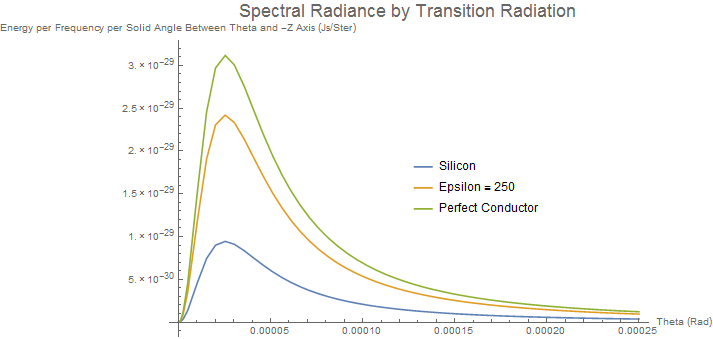
\includegraphics[scale=0.5]{dWdomega.PNG}
\caption{This figure shows the spectral radiance for the transition radiation $\frac{\mathrm{d}W}{\mathrm{d} \omega \mathrm{d} \Omega}$ for angle $\theta$ with respect to the normal of the foil.}
\end{center}
\end{figure}

For a non-perfect conductor, integrating over all of $\phi$ and over the $\theta$ that is covered by the camera lens $\theta_a$ is given by

\begin{equation}
\frac{dW} {d \omega} =2 \pi \int\limits_0^{\theta_{a}} \sin \theta \frac{e^{2} \beta^{2} \sin^2 \theta \cos^2 \theta} {\pi^{2} c (1-\beta^{2} \cos^2 \theta)^{2}} \times (\frac{(\epsilon -1) (1-\beta^{2}+\beta \sqrt{\epsilon-\sin^2 \theta})} {(1+\beta \sqrt{\epsilon-\sin^2 \theta}) (\epsilon \cos \theta + \sqrt{\epsilon- \sin^2 \theta})})^{2} \mathrm{d} \theta
\end{equation}

Doing the same integration to a perfect conductor gives

\begin{equation}
\frac{dW} {d \omega} =2 \pi \int\limits_0^{\theta_{a}} \sin \theta \frac{e^{2} \beta^{2} \sin^2 \theta} {\pi^{2} c (1-\beta^{2} \cos^2 \theta)^{2}} \mathrm{d} \theta
\end{equation}

This integration for the perfect conductor is done exactly in [2] and gives the following
\begin{equation}
\frac{dW} {d \omega} (\theta_{a}) =\frac{e^{2}} {2 \pi c} \times (\frac{2(1-\beta^{2}) \cos \theta_{a}}{1-\beta^2 \cos^2 \theta_{a}}+\frac{1+\beta^{2}}{\beta} \ln{\frac{(1-\beta \cos \theta_{a})(1+\beta)}{(1+\beta \cos \theta_{a})(1-\beta)}}-2)
\end{equation}

Fig. 2 gives the total energy collected by the camera that covers an angle $\theta_a$.

\begin{figure}
\begin{center}
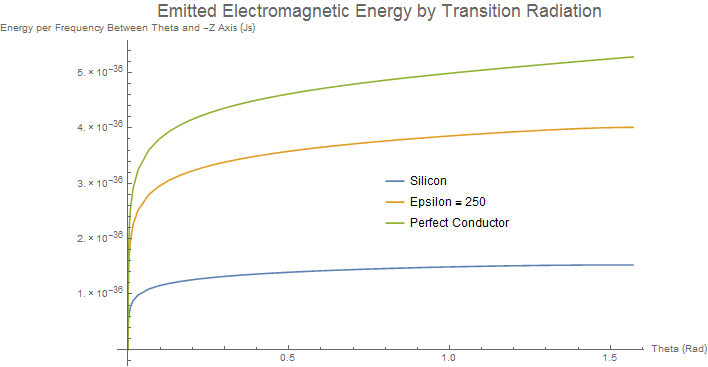
\includegraphics[scale=0.5]{Energy2.PNG}
\caption{This figure shows the total energy per electron collected by the camera that covers an angle $\theta$.}
\end{center}
\end{figure}

where $\theta_a$ is the angle that the camera covers. Assuming that we know the results above, we can now attempt to back out the number of photons emitted in the visible spectrum. Notice that the above equations are independent of frequency, thus each frequency in the visible range emits the same amount of energy.

\begin{equation}
\mathrm{d} W=n \hbar \mathrm{d} \omega
\end{equation}

\begin{equation}
n=\frac{\mathrm{d} W}{\mathrm{d} \omega} \frac{1}{\hbar}
\end{equation}

\begin{equation}
n_{visible}=\frac{\mathrm{Total Visible Energy}}{\mathrm{Average Energy per Photon}}=\frac{\mathrm{d} W}{\mathrm{d} \omega} \frac{\omega_2 - \omega_1}{\hbar \omega_{avg}}
\end{equation}

The results of the calculation are shown in Fig. 3 for given input parameters such as the distance from the camera to the interaction point $d$, diameter of the lens $a$, $\gamma$, and various dielectric constants $\epsilon$.

\begin{figure}
\begin{center}
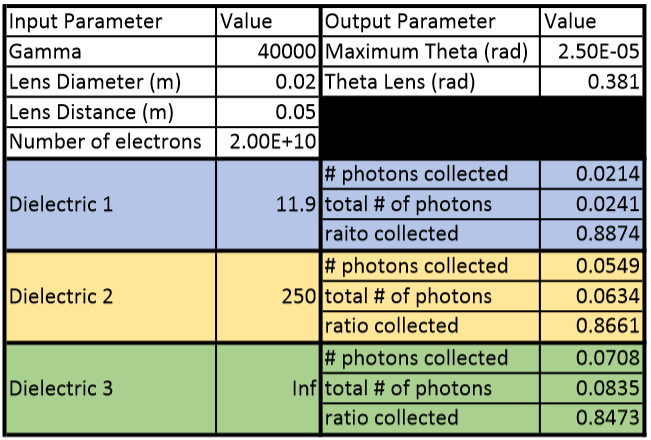
\includegraphics[scale=0.5]{TransData.PNG}
\caption{This table shows the input parameters and various output paramters such as the number of photons emitted by transition radiation (per electron) as well as other relevant parameters.}
\end{center}
\end{figure}

\section{Diffraction Radiation}

The diffraction radiation equation can be found in the Accelerator Handbook [2]. This equation applies to a circular hole in a foil, and it is the energy emitted per electron at a distance $r$ from the center of the hole of radius $a$. It is a function of the transition radiation $\frac{dW_{TR}} {d \Omega d \omega}$. Thus, I cannot compute this until I solve resolve my problems with transition radiation.

\begin{equation}
\frac{dW} {d \Omega d \omega}=\frac{dW_{TR}} {d \Omega d \omega} [J_{0}(ka \sin \theta)^{2}+(\frac {r}{a})^{2} J_{1}(ka \sin \theta)^{2}]
\end{equation}

where $k=\frac{\omega}{c}$. Thus, the differential diffraction radiation does depend on frequency.

\begin{equation}
\frac{dW} {d \Omega d \omega}=\frac{dW_{TR}} {d \Omega d \omega} [J_{0}(\frac {\omega a}{c} \sin \theta)^{2}+(\frac {r}{a})^{2} J_{1}(\frac {\omega a}{c} \sin \theta)^{2}]
\end{equation}

Integrating around all of d$\phi$ and also d$\theta$ and d$\omega$ gives

\begin{equation}
W(r)= 2 \pi \int_{\omega_{1}}^{\omega_{2}} \int_{0}^{\theta_{a}} \sin \theta \frac{dW_{TR}} {d \Omega d \omega} [J_{0}(\frac {\omega a}{c} \sin \theta)^{2}+(\frac {r}{a})^{2} J_{1}(\frac {\omega a}{c} \sin \theta)^{2}] \mathrm{d} \theta \mathrm{d} \omega
\end{equation}

The energy emitted per electron is a function of $r$, the distance from the center of the hole. Thus, we must know the density of electrons at each point. I will have to look up exactly what the density function for a bunch of particles, but I remember it is some form of a Gaussian. Let's say the density is radially symmetric, $\rho (r)$ and the center of the beam travels in the center of the hole. Then the differential energy from the emitted visible photons at a distance $r$ from the center in the region d$r$ is

\begin{equation}
\mathrm{d}W_{total}(r)=2 \pi \rho (r) W(r) \mathrm{d}r
\end{equation}

Using the equation in the previous section, the number of photons emitted d$n$ at a distance $r$ in s small interval d$r$ is given by

\begin{equation}
\mathrm{d}n=\mathrm{d} W_{total} \frac{1}{\hbar \omega_{avg}}
\end{equation}

Finally, integrating over $r$ gives the total number of photons

\begin{equation}
n=\int_0^{\infty} \mathrm{d} W_{total} \frac{1}{\hbar \omega_{avg}}
\end{equation}

\section{Diffraction Radiation of a Slit}

\begin{equation}
\frac{\mathrm{d} N}{\mathrm{d} \Omega}=-\frac{\alpha}{2\lambda^2} \frac{\mathrm{d} \lambda}{\lambda} \frac{e^{-af}}{f^2+k_{y}^{2}} ((e^{2yf}+e^{-2yf})-2 \sin (ak_y+\Phi))
\end{equation}

\begin{equation}
k=\frac{2 \pi}{\lambda},
k_x=k \sin \theta \cos \phi,
k_y=k \sin \theta \sin \phi
\end{equation}
\begin{equation}
f=\sqrt{k_{x}^{2}+\eta^2},
\eta^2=\frac{k^2}{\beta^2 \gamma^2}
\end{equation}
\begin{equation}
f^2+k_{y}^{2}=-2fk_y \sin \Phi = (f^2-k_{y}^{2}) \cos \Phi
\end{equation}

\begin{equation}
S(x)=\frac{1}{\sqrt{2 \pi} \sigma_y} e^{-(y-y_0)^2/2 \sigma_{y}^{2}}
\end{equation}

\begin{equation}
\frac{\mathrm{d} N}{\mathrm{d} \Omega}=-\frac{\alpha}{2\lambda^2} \frac{\mathrm{d} \lambda}{\lambda} \frac{e^{-af}}{f^2+k_{y}^{2}} (e^{2 f^2 \sigma_{y}^{2}}(e^{2y_0 f}+e^{-2y_0 f})-2 \sin (ak_y+\Phi))
\end{equation}

%\begin{equation}
%\frac{\mathrm{d} N}{\mathrm{d} \Omega}(\phi=+/- \pi/2)=-\frac{\alpha}{4 \pi^2} \frac{\mathrm{d} \lambda}{\lambda} \frac{e^{-2 \pi a/ \lambda \gamma}}{\theta^2+1/ \gamma^2} (e^{8 \pi^2 \sigma_{y}^{2}/\gamma^2 %\lambda^2}-2 \sin{\frac{2 \pi a \theta}{\lambda}+\Phi}})
%\end{equation}


\section{Optical Diffraction Radiation Part III}

The spectral intensity $\frac{dI}{d \omega}$ for optical diffraction radiation from a flat metal foil with an impact parameter of $\vec{u}=u_x \hat{i}+u_y \hat{y}$ is given by

\begin{equation}
\frac{dI}{d \omega}(u_x,u_y,\omega)=\frac{e^2}{\pi^2 c \beta^2} \frac{1}{(\gamma \lambda)^2} \frac{N}{2 \pi \sigma_x \sigma_y} \int \int K_{1}^{2}(\frac{1}{\gamma \lambda} \sqrt{(u_x-x)^2+(u_y-y)^2}) e^{-(\frac{x^2}{2 \sigma_{x}^{2}}+\frac{y^2}{2 \sigma_{y}^{2}})} dx dy
\end{equation}

where $\sigma_x$ and $\sigma_y$ are the beam sizes in the $x$ and $y$ directions, respectively, $N$ is the total number of electrons, $\lambda$ is the wavelength, and $K_1^{2}$ is the modified Bessel function. In the analysis, it is important to analyze both the $x$ and $y$ projections, which are $\frac{dI_x}{d \omega}$ and $\frac{dI_y}{d \omega}$, respectively.

\begin{equation}
\frac{dI_x}{d \omega}(u_x, \omega)=\frac{e^2}{\pi^2 c \beta^2} \frac{1}{(\gamma \lambda)^2} \frac{N}{2 \pi \sigma_x \sigma_y} \int_{u_y=a}^{\infty} \int \int K_{1}^{2}(\frac{1}{\gamma \lambda} \sqrt{(u_x-x)^2+(u_y-y)^2}) e^{-(\frac{x^2}{2 \sigma_{x}^{2}}+\frac{y^2}{2 \sigma_{y}^{2}})} dx dy du_y
\end{equation}

where $a$ is the impact parameter.

\begin{equation}
\frac{dI_y}{d \omega}(u_y,\omega)=\frac{e^2}{\pi^2 c \beta^2} \frac{1}{(\gamma \lambda)^2} \frac{N}{2 \pi \sigma_x \sigma_y} \int \int \int K_{1}^{2}(\frac{1}{\gamma \lambda} \sqrt{(u_x-x)^2+(u_y-y)^2}) e^{-(\frac{x^2}{2 \sigma_{x}^{2}}+\frac{y^2}{2 \sigma_{y}^{2}})} dx dy d_ux
\end{equation}

Also, the total number of visible photons $n$ emitted due to diffraction radiation is given by

\begin{equation}
n=\frac{1}{4 \pi \epsilon_0} \frac{e^2}{\pi^2 c \beta^2 \hbar \omega_{avg}} \frac{1}{(\gamma \lambda)^2} \frac{N}{2 \pi \sigma_x \sigma_y} \int_{\omega_1}^{\omega_2} \int_{a}^{\infty} \int \int \int K_{1}^{2}(\frac{1}{\gamma \lambda} \sqrt{(u_x-x)^2+(u_y-y)^2}) e^{-(\frac{x^2}{2 \sigma_{x}^{2}}+\frac{y^2}{2 \sigma_{y}^{2}})} dx dy du_x du_y d \omega
\end{equation}

where $\omega_1$ and $\omega_2$ are the lower and upper frequencies of visible light, respectively, $\omega_{avg}$ is the average visible frequency, and the factor $\frac{1}{4 \pi \epsilon_0}$ is multiplied to the integral.

\begin{figure}
\begin{center}
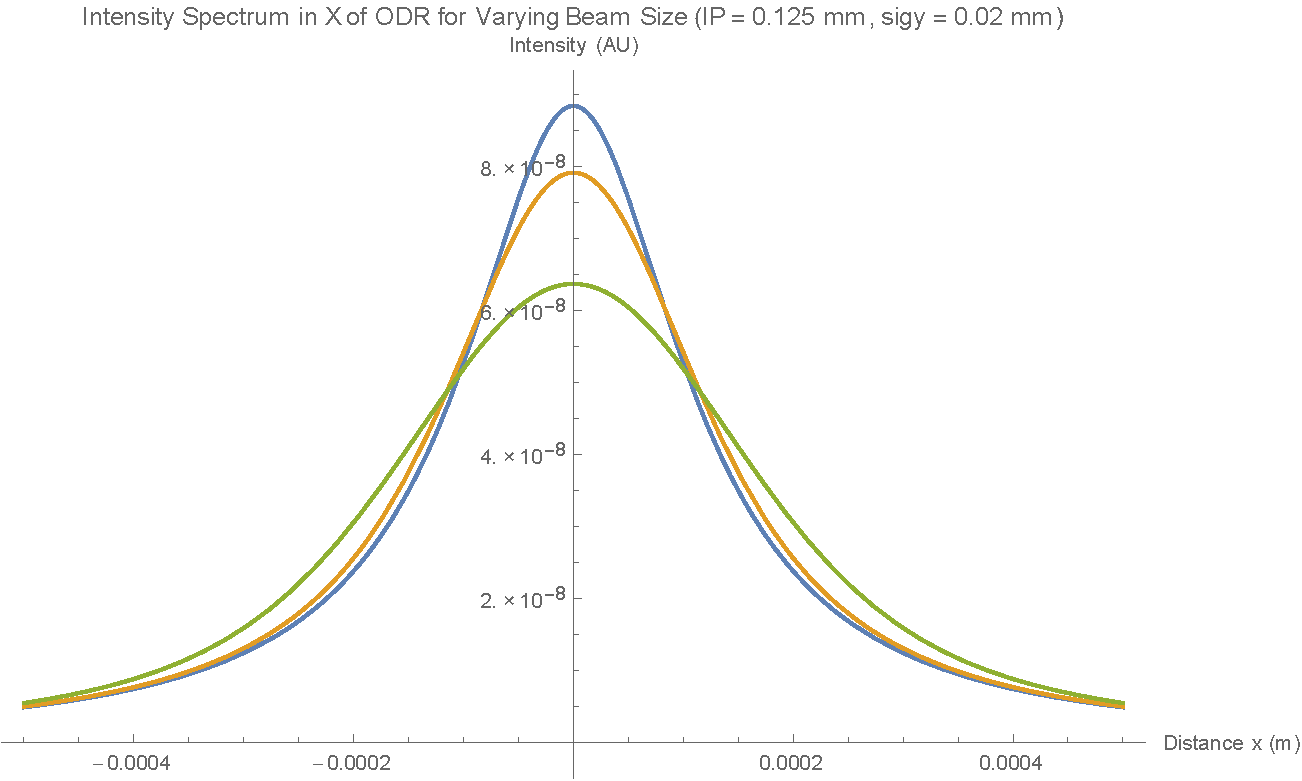
\includegraphics[scale=0.5]{figures/ODR_IntensityX.PDF}
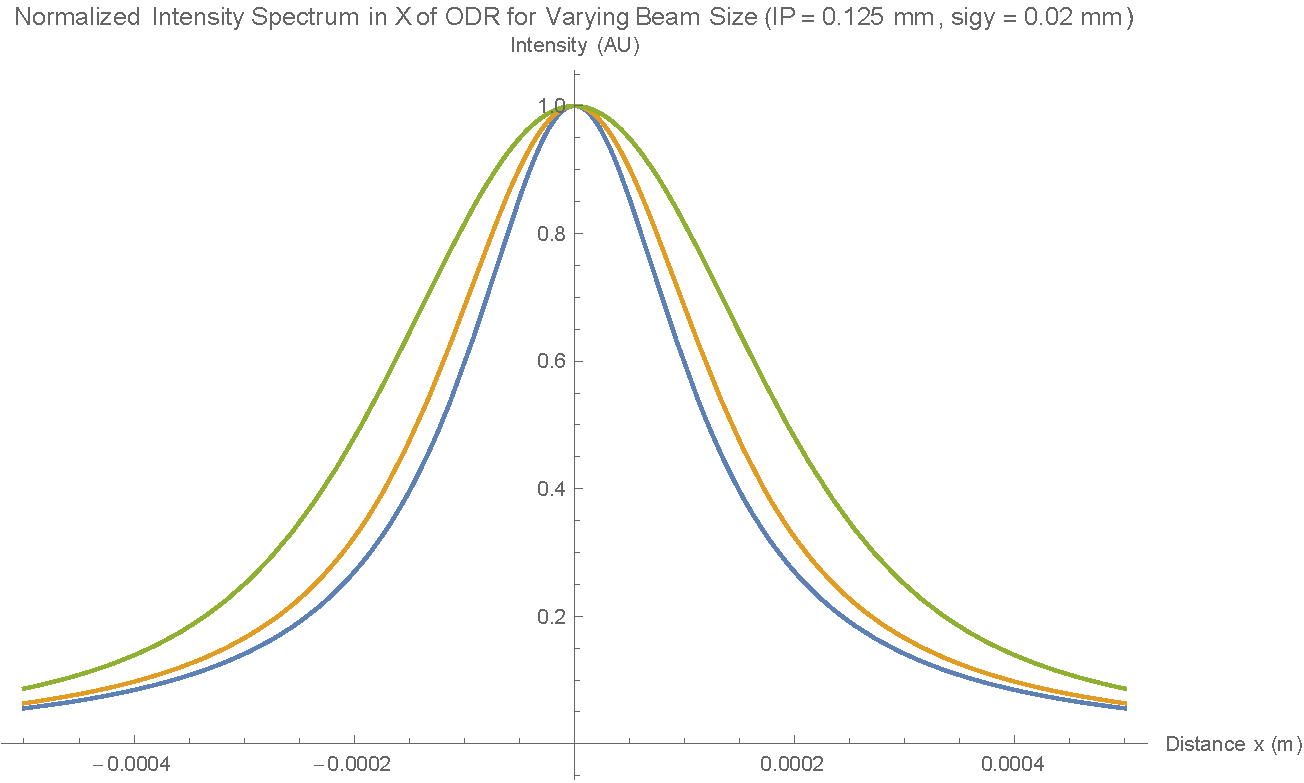
\includegraphics[scale=0.5]{figures/ODR_Norm_IntensityX.PDF}
\caption{INSERT CAPTION HERE}
\end{center}
\end{figure}

\begin{figure}
\begin{center}
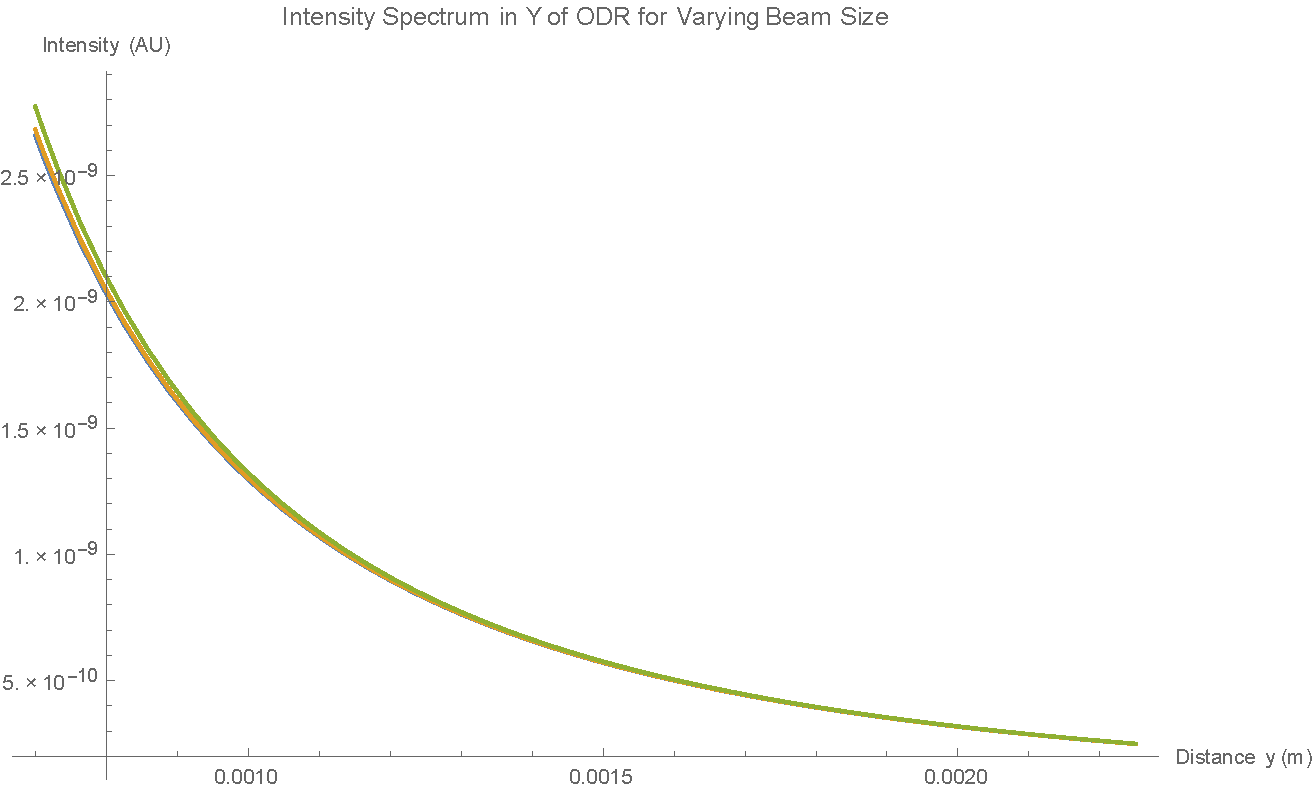
\includegraphics[scale=0.5]{figures/ODR_IntensityY.PDF}
\caption{INSERT CAPTION HERE}
\end{center}
\end{figure}

\begin{figure}
\begin{center}
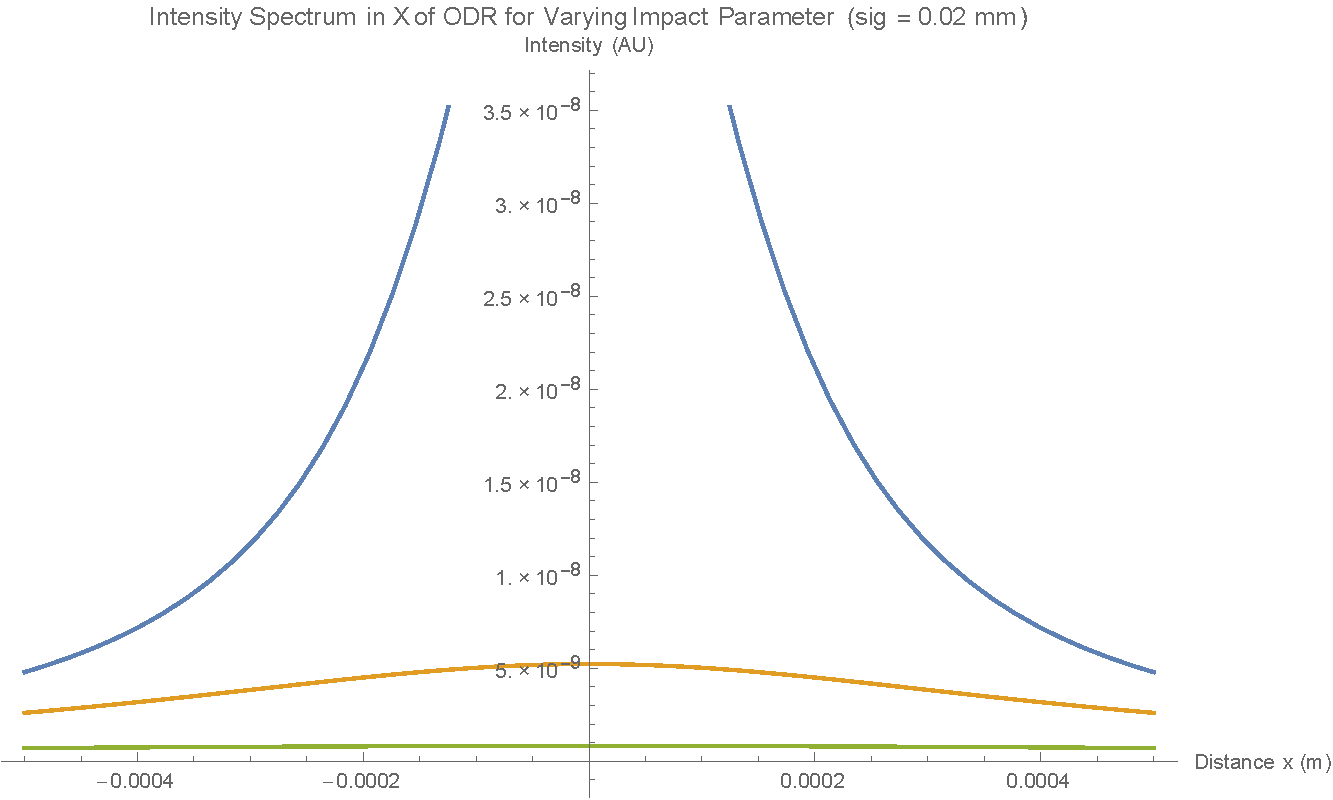
\includegraphics[scale=0.5]{figures/ODR_IntensityX_IP.PDF}
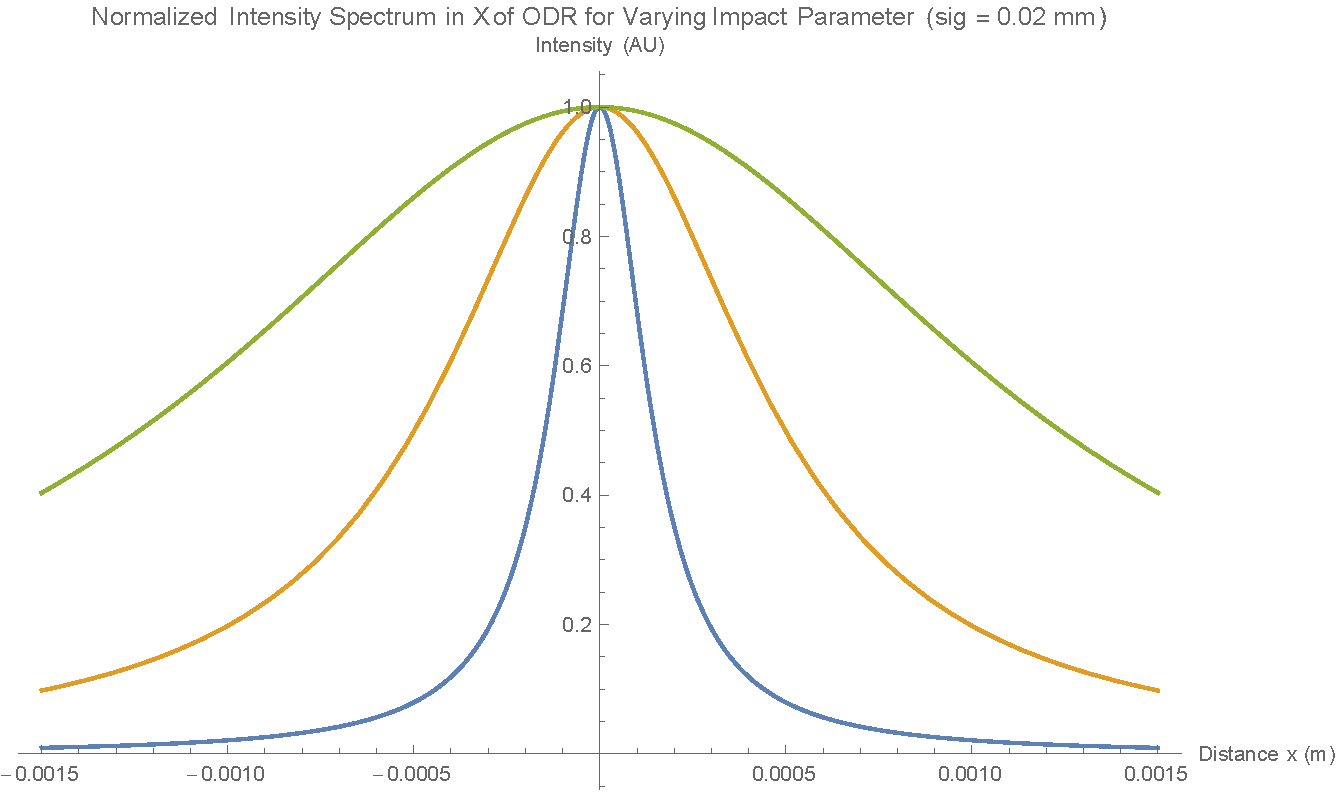
\includegraphics[scale=0.5]{figures/ODR_Norm_IntensityX_IP.PDF}
\caption{INSERT CAPTION HERE}
\end{center}
\end{figure}

\begin{figure}
\begin{center}
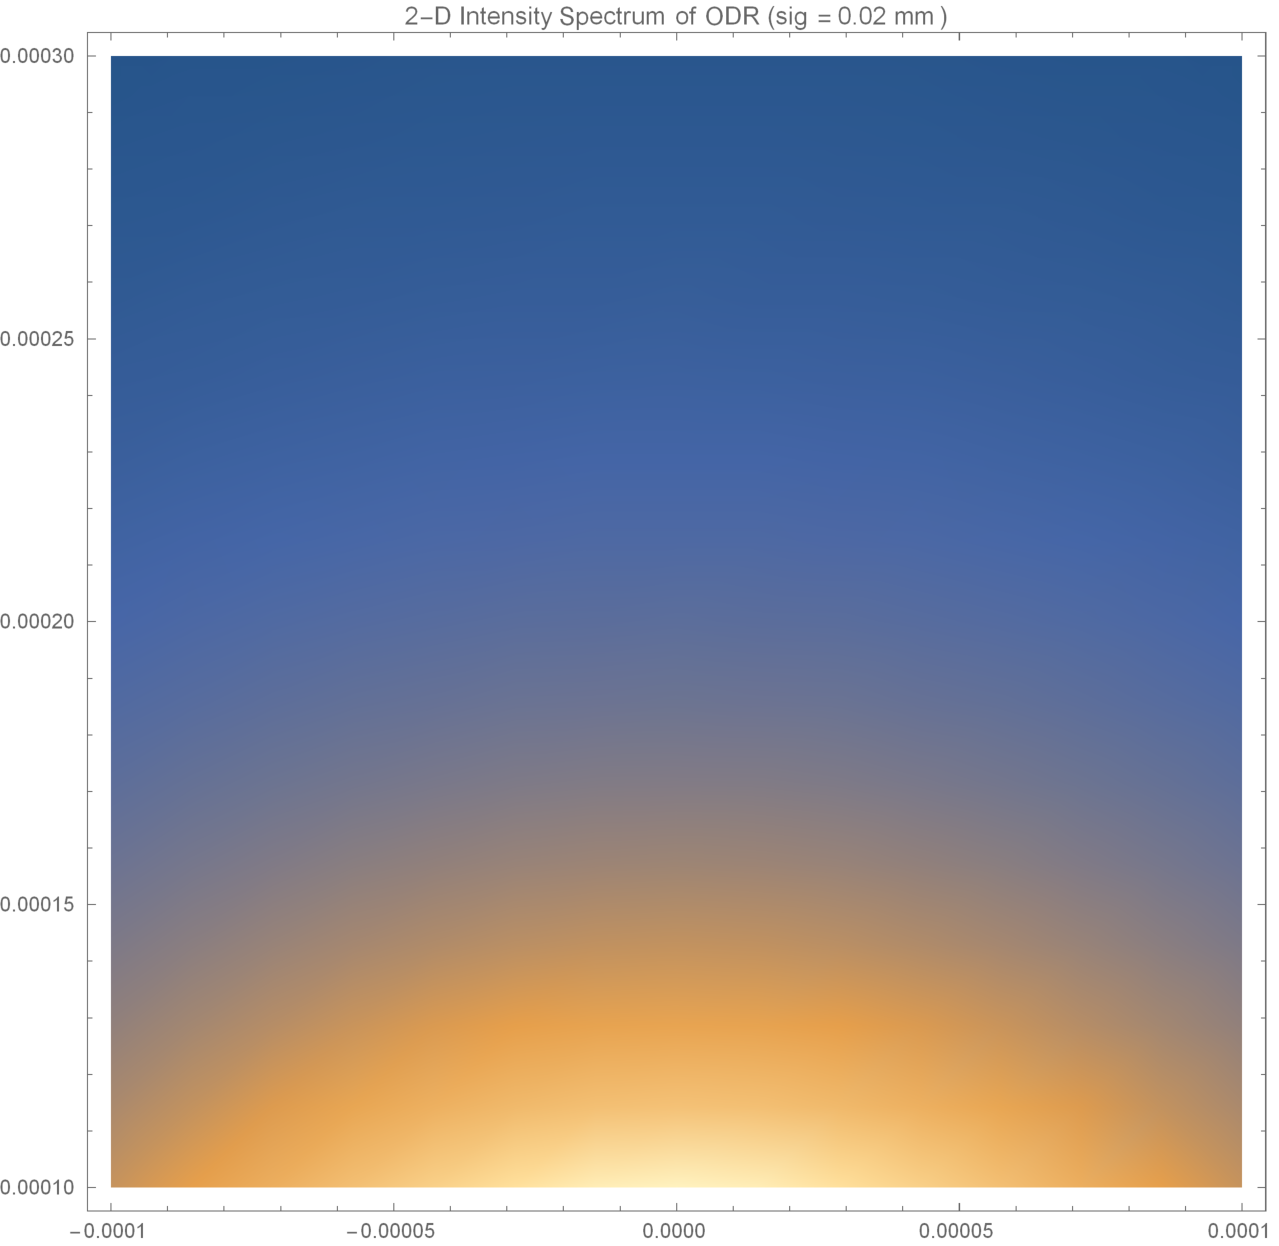
\includegraphics[scale=0.5]{figures/ODR_2D_Intensity.PDF}
\caption{INSERT CAPTION HERE}
\end{center}
\end{figure}

\begin{figure}
\begin{center}
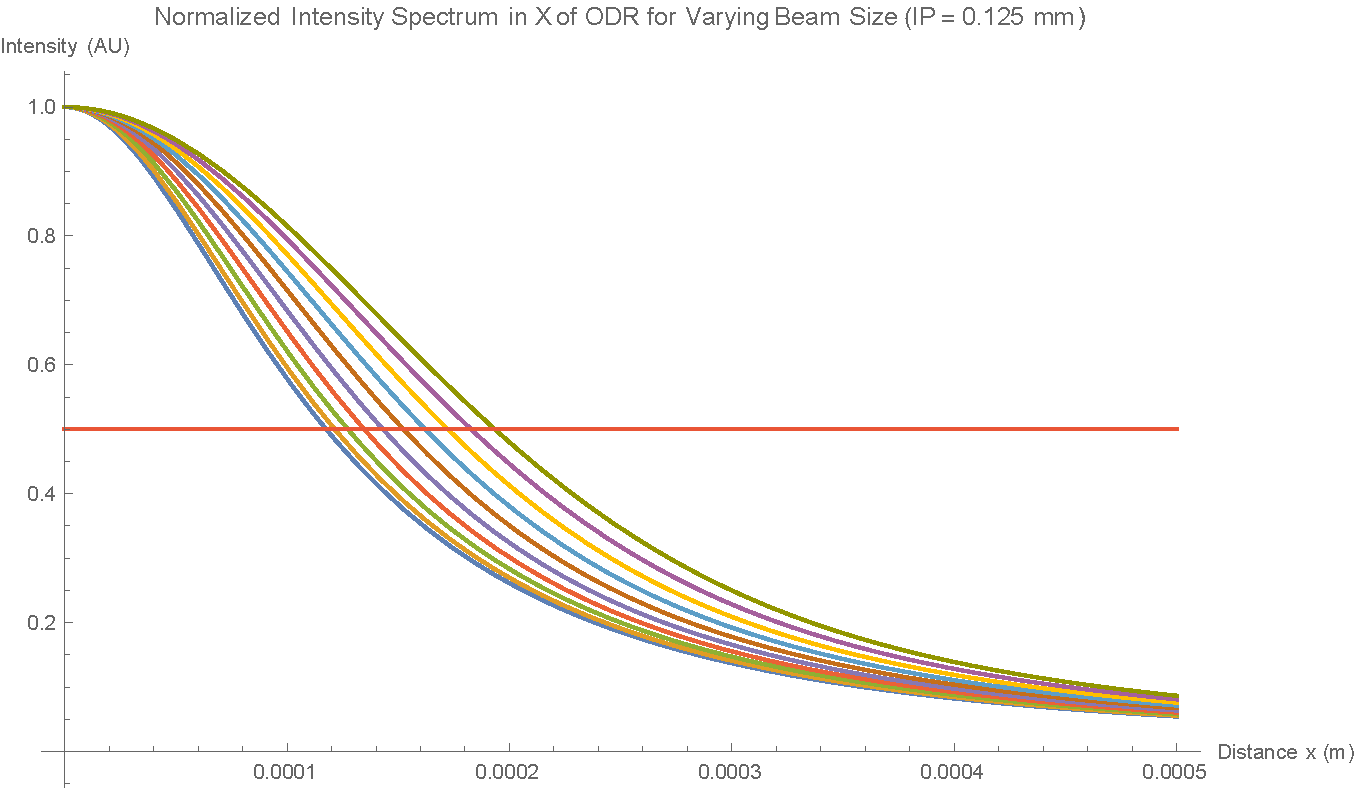
\includegraphics[scale=0.5]{figures/ODR_Norm_IntensityX_125.PDF}
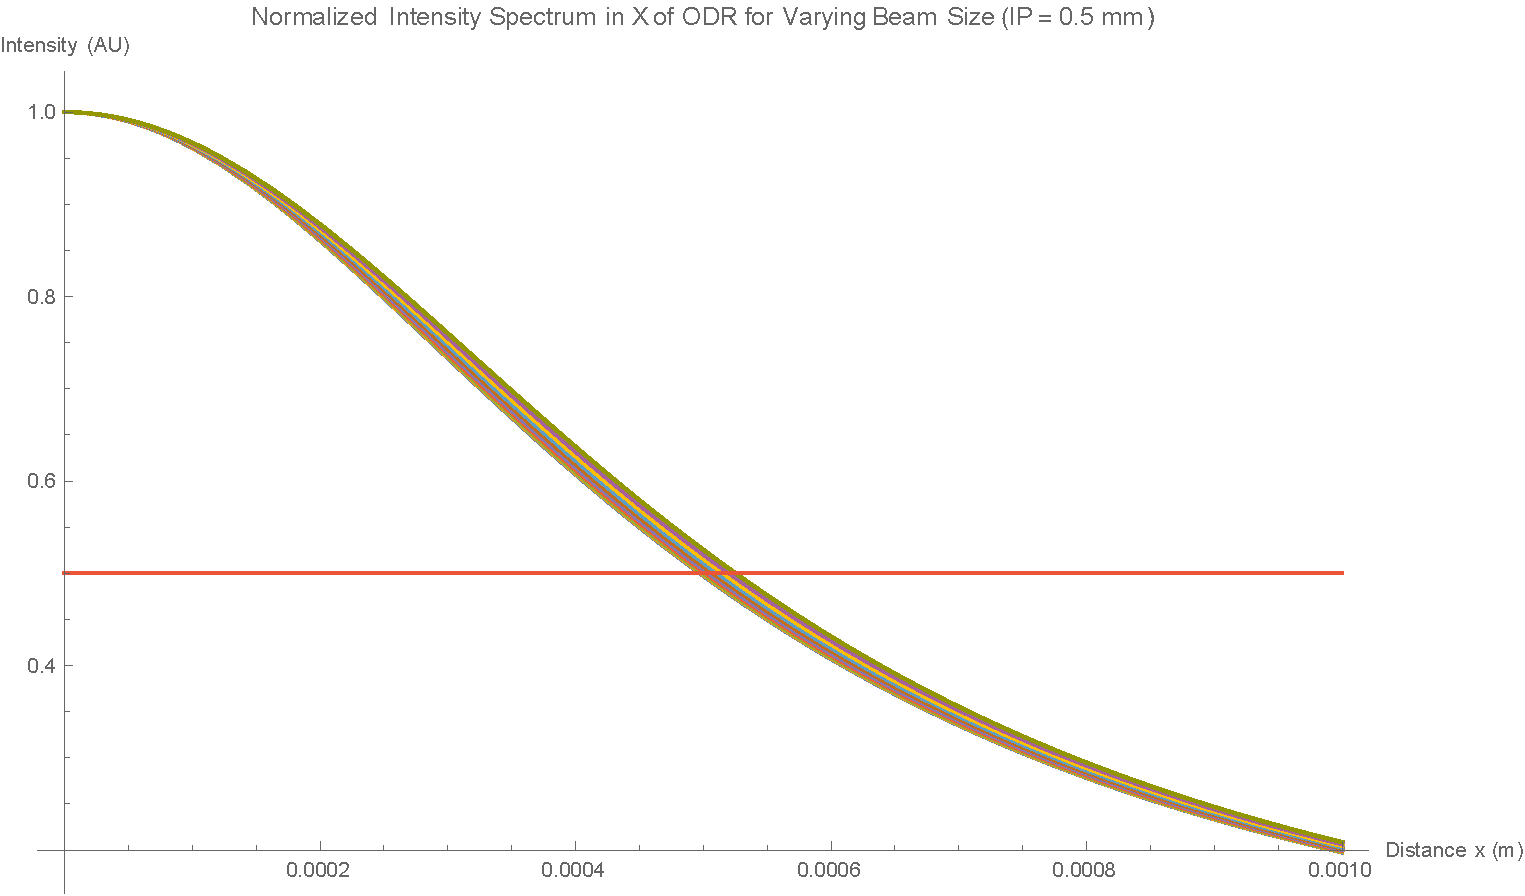
\includegraphics[scale=0.5]{figures/ODR_Norm_IntensityX_500.PDF}
\caption{INSERT CAPTION HERE}
\end{center}
\end{figure}

\begin{figure}
\begin{center}
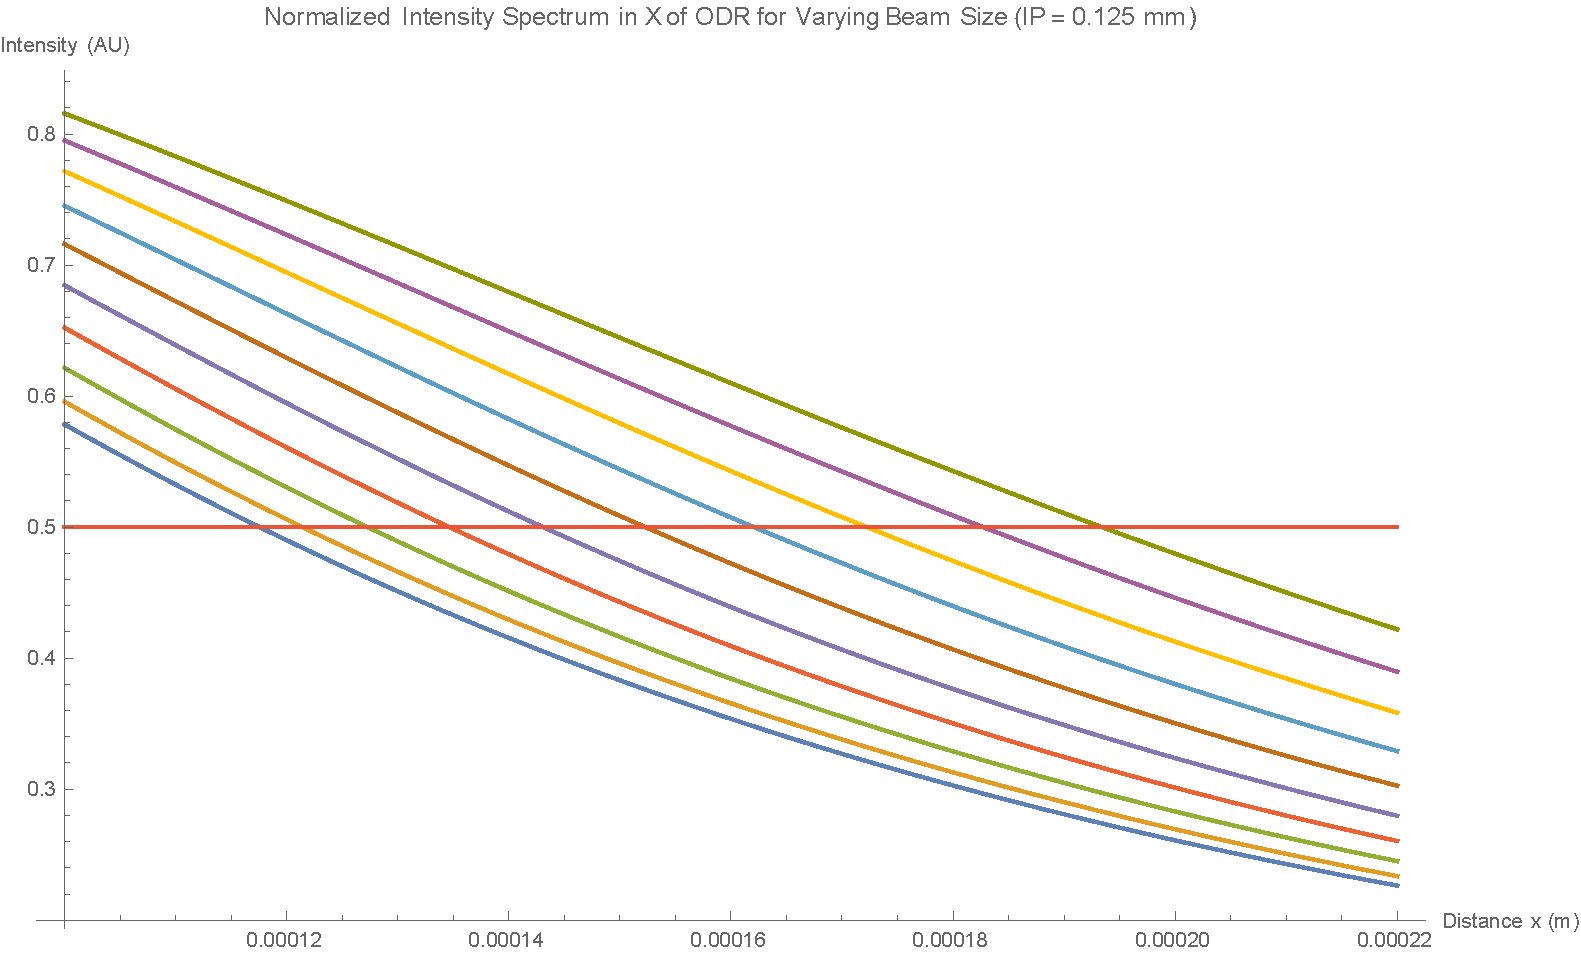
\includegraphics[scale=0.5]{figures/ODR_Norm_IntensityX_125_zoom.PDF}
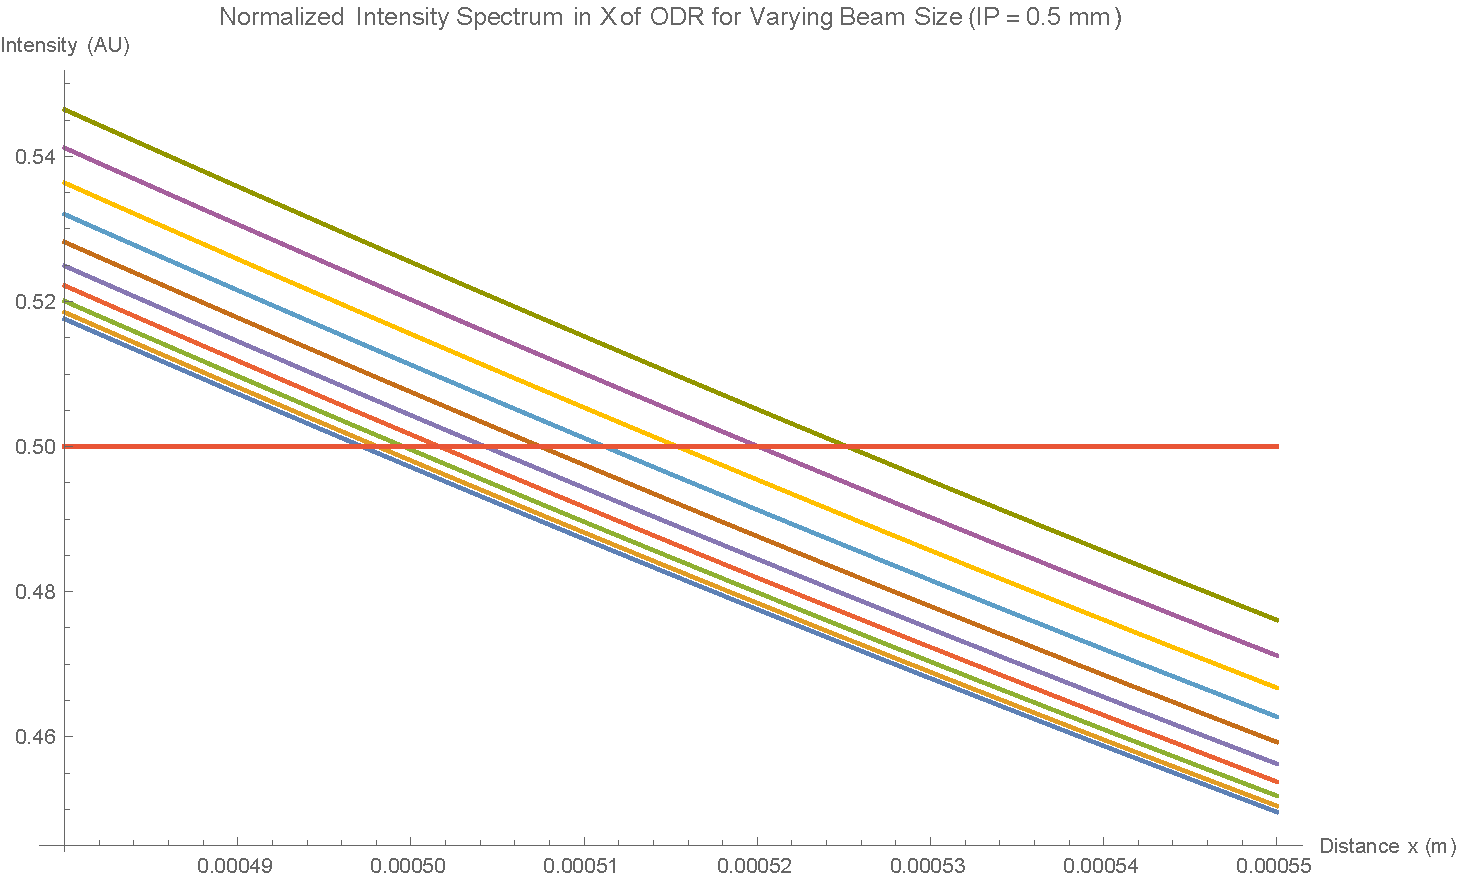
\includegraphics[scale=0.5]{figures/ODR_Norm_IntensityX_500_zoom.PDF}
\caption{INSERT CAPTION HERE}
\end{center}
\end{figure}





\section{Thermal Radiation}

Stupakov's equation for the amount of energy $P$ deposited by a beam in a foil can be found in his paper [3]. In these equations, $Q$ is the total charge of the bunch, $X$ and $Y$ are the dimensionless coordinates $X=\frac{x}{\sigma_z}$ and $Y=\frac{y}{\sigma_z}$, respectively, and $s_x$ and $s_y$ are the dimensionless beam sizes $s_x=\frac{\sigma_x}{\sigma_z}$ and $s_y=\frac{\sigma_y}{\sigma_z}$, respectively. Also, $\Omega=\frac{\omega \sigma_z}{c}$ and $\rho$ is the radius. I am unsure what $\omega$ is, it appears to be the constant of integration when the author does Fourier Transforms. We start with the equation for energy at given coordinates $X$ and $Y$ from the center of the interaction point.

\begin{equation}
P=\frac{Q^2}{4 \pi^{3} \sigma_{x}^{2} \sigma_{y}^{2}} H(X,Y,\Omega,s_x,s_y)
\end{equation}

where

\begin{equation}
H(X,Y,\Omega,s_x,s_y)=\int_0^{\infty} \Omega \mathrm{d} \Omega [|R_{x} (X,Y,\Omega,s_x,s_y)|^2+|R_{y} (X,Y,\Omega,s_x,s_y)|^2]
\end{equation}

where

\begin{equation}
R_{x} (X,Y,\Omega,s_x,s_y)=- \int \mathrm{d} \rho \mathrm{d} \phi \sin \phi \exp{(-\frac{(X+\rho \cos \phi)^2}{2 s_{x}^{2}}-\frac{(Y+\rho \sin \phi)^2}{2 s_{y}^{2}}-\frac{\Omega^2}{2}+i \Omega \rho)}
\end{equation}

and

\begin{equation}
R_{y} (X,Y,\Omega,s_x,s_y)= \int \mathrm{d} \rho \mathrm{d} \phi \cos \phi \exp{(-\frac{(X+\rho \cos \phi)^2}{2 s_{x}^{2}}-\frac{(Y+\rho \sin \phi)^2}{2 s_{y}^{2}}-\frac{\Omega^2}{2}+i \Omega \rho)}
\end{equation}

While attempting to integrate these via Mathematica, it has some difficulties saying that the functions are "too oscillatory" to integrate precisely. Matlab is even more of a nightmare. Nevertheless, I proceed with my calculation. I am unsure if the remainder of this calculation is correct, but it was worth a try. Assuming I have calculated the energy $P$ correctly at each coordinate, then the temperature change associated with that is given by the simple formula

\begin{equation}
P=k \times m \times \Delta T=k \times m \times (T(X,Y)-T_0)
\end{equation}

where $k$ is the thermal constant of the material, $m$ is the mass, $T(X,Y)$ is the temperature as a function of position on the foil and $T_0$ is the room temperature. Each small element of mass d$m$ will receive a small amount of energy d$P$.

\begin{equation}
\mathrm{d}P=k \mathrm{d}m (T(X,Y)-T_0)
\end{equation}

Solving for $T=T(X,Y)$ gives

\begin{equation}
T=T_0+\frac{1}{k} \frac{\mathrm{d}P}{\mathrm{d}m}=T_0+\frac{1}{k \rho_0} \frac{\mathrm{d}P}{\mathrm{d}V}=T_0+\frac{1}{k \rho_0 d_0} \frac{\mathrm{d}P}{\mathrm{d}A}=T_0+\frac{1}{k \rho_0 d_0} \frac{\mathrm{d}P}{\mathrm{d}X \mathrm{d}Y}
\end{equation}

where $\rho_0$ is the material density and $d_0$ is the skin depth. I am unsure if I have used this skin depth properly.

The differential of intensity $I$ (energy per time) per solid angle per area per wavelength is given by

\begin{equation}
\frac{\mathrm{d}I}{\mathrm{d} \Omega \mathrm{d}A \mathrm{d} \lambda}=\frac{2hc^2}{\lambda^5} \frac{1}{\exp{\frac{hc}{k_b T}}-1}
\end{equation}

After integrating over $\phi$ for the full 2$\pi$ radians, we can integrate over $\theta$ with the range that the camera covers $\theta_a$ and over the visible spectrum.

\begin{equation}
\frac{\mathrm{d}I}{\mathrm{d}A}=2 \pi \int_{\lambda_1}^{\lambda_2} \int_0^{\theta_a} \sin \theta \frac{\mathrm{d}I}{\mathrm{d} \theta \mathrm{d} \lambda} \mathrm{d} \theta \mathrm{d} \lambda
\end{equation}

We can integrate this function over the entire area.

\begin{equation}
I=\int_{-\infty}^{\infty} \int_{-\infty}^{\infty} \frac{\mathrm{d}I}{\mathrm{d}A} \mathrm{d}X \mathrm{d}Y
\end{equation}

Thus we have the energy per unit time. Finally, we can find the number of photons $n$ per unit time simply by differentiating $E=\frac{hc}{\lambda} n$ and using the average wavelength $\lambda_{avg}$.

\begin{equation}
\frac{\mathrm{d}n}{\mathrm{d}t}=\frac{\lambda_{avg}}{hc} I
\end{equation}

Thus we have the photon rate. Mathematica will probably have fun with this calculation....

\section{Thermal Radiation II}

The total power $P$ delivered to the foil from the beam is given by the following equation where we assume a worst case scenario of a foil of thickness $\delta=25 \mu m$.

\begin{equation}
P=-\rho \frac{\mathrm{d} E}{\mathrm{d} x} \times N \times PRR \times \delta
\end{equation}

where $-\rho \frac{\mathrm{d} E}{\mathrm{d} x}$ is the energy loss of an electron per unit length of the foil, $N$ is the number of electrons in the bunch, and $PRR$ is the pulse repititon rate. Plugging in numbers for titanium gives the amount of power delivered over the small area of the foil.

\begin{equation}
P_{Ti}=7.17 \times 10^6 \frac{eV}{cm} \times 10^{10} \times 10 Hz \times 25 \times 10^{-4} cm \times \frac{1.6 \times 10^{-19} J}{1 eV}=0.0002868 W
\end{equation}

The amount of power per unit volume, assuming a beam size of $ \sigma = 25 \mu m$, is

\begin{equation}
S=\frac{P}{V}
\end{equation}

and for the titanium is

\begin{equation}
S_{Ti}=\frac{0.0002868 W}{\pi (20 \times 10^{-4})^2 \times 25 \times 10^{-4} cm^3}=9129 W/cm^3
\end{equation}

We will now compare the power input into the foil with the power radiated away due to temperature differences between the foil $T_1$ and the surroundings $T_2=300 K$.

\begin{equation}
q''_r=\epsilon \sigma (T_{1}^{4}-T_{2}^{4})
\end{equation}

where $\sigma$ is the Stefan-Boltzmann constant, $\epsilon$ is the emissivity of the foil, and $q''_r$ is the power emitted per unit area. For this analysis, we will assume that the foil is $50 \degree C$ below its melting point to obtain a worst case scenario. For titanium, this gives

\begin{equation}
q''_{r Ti}=0.2 \times 5.77 \times 10^{-12} (1900^{4}-300^{4})=15.03 W/cm^2
\end{equation}

And multiplying by the area gives

\begin{equation}
A=\pi \sigma^{2}=\pi (20 \times 10^{-4})^2=1.257 \times 10^{-5} cm^2
\end{equation}

\begin{equation}
P_{r Ti}=q''_{r Ti} \times A=0.000189 W
\end{equation}

Since the power radiated away is much less than the power deposited by the beam, most of the energy must be conducted away. We can start by searching for a steady-state solution to this problem assuming constant power being deilvered to the foil and no radiative heat loss. The difference in temperature between the foil $T_o$ and and the surroundings $T_i$ is given by

\begin{equation}
T_o-T_i=\frac{S \sigma^{2}}{4 K}
\end{equation}

where $k$ is the thermal conductivity of the foil. For titanium, this gives

\begin{equation}
(T_o-T_i)_{Ti}=\frac{9129 W/cm^3 (20 \times 10^{-4})^{2}}{4 \times 0.219 W/cm K}=0.0417 K
\end{equation}

Next, we can find the steady-state temperature difference $\Delta T$ (again assuming no radiative heat loss) between the spot where the beam deposits its energy and the remainder of the foil. We will also assume that the foil has a radius of $r_o=1.27 cm$. 

\begin{equation}
\Delta T=P' \frac{ln(\frac{r_o}{\sigma})}{2 \pi k}
\end{equation}

For titanium, this gives

\begin{equation}
\Delta T_{Ti}=\frac{0.0002868}{25 \times 10^{-6}} W/m \frac{ln(\frac{1.27 cm}{20 \times 10^{-4} cm})}{2 \pi 21.9 W/mk}=0.538 K
\end{equation}

Repeating the method for silicon after gives the following results

\begin{equation}
P_{Si}= 0.000155 W, q''_{r Si}=26.77 W/cm^2 , P_{r Si}=0.000337 W , (T_o-T_i)_{Si}=0.00334 K , \Delta T_{Si}=0.0430 K
\end{equation}

Now, in order to find the temperature profile as a function of $r$ and $t$, we use the heat equation for radial symmetry. We are assuming only conduction (without thermal radiation) in order to simplify the equation and to provide an upper bound.

\begin{equation}
\rho c_p \frac{\partial T}{\partial t}=\frac{1}{r} \frac{\partial}{\partial r} (k r \frac{\partial T}{\partial r})
\end{equation}

where $\rho$ is the density, $c_p$ is the specific heat, and $k$ is the thermal conductivity. The general solution to this equation is as follows.

\begin{equation}
T(r,t)=Ae^{-\alpha t} (c_1 J_0(\sqrt{\frac{\alpha \rho c_p}{k}}r)+c_2 Y_0(\sqrt{\frac{\alpha \rho c_p}{k}}r))
\end{equation}

where $J_0$ and $Y_0$ are Bessel function of the first and second kind, respectively, and $A$, $c_1$, and $c_2$ are arbitrary constants and $\alpha$ is related to how quickly the temperature decreases due to conduction. We must solve the equation for the following boundary conditions

\begin{equation}
T(0 \le r \le \sigma,0)=T_h, T(0,a)=T_0
\end{equation}

where $\sigma$ is the spot size of the beam, $T_h$ is the temperature immediately after the beam deposits energy into the foil, $a$ is the radius of the foil, and $T_0$ is the boundary temperature. I am currently figuring out how to apply the boundary conditions...

\section*{References}
\begin{enumerate}[{[}1{]}]
\item http://inspirehep.net/record/562218/files/slac-r-576.pdf
\item Accelerator Handbook
\item http://slac.stanford.edu/pubs/slacpubs/15500/slac-pub-15729.pdf

\end{enumerate}

\end{document}
